\chapter{Quark Spectral Functions in QCD}\label{chap:results}
This chapter summarizes the main part of our work. The goal  is to find a K\"all\'{e}n-Lehmann spectral representation of the quark propagator by iteratively solving the corresponding Dyson-Schwinger equation. Employing the KL spectral representation of the quark and gluon propagators allows for a perturbative treatment of the occurring loop diagram at the expense of additional spectral integrals for every propagator, and basically also for every higher $n$-point function\footnote{Whereas axiomatic approaches to QFT predict their existence in general, there has not yet been a lot of work on spectral representations for higher order $n$-point functions. } involved in the computation. The spectral renormalization scheme put forward in \cite{Horak2019,Wink2020,HorakPawlowskiWink2020} provides a well suited  framework for a practical numerical implementation of our problem while maintaining all underlying symmetries of the theory at hand.\\
 The first part of this chapter provides a detailed introduction to the general methodology of the spectral renormalization scheme. The aim  is to guide the reader through the most important steps of the conducted calculations using the concrete example of the quark DSE, focusing on the conceptually most important steps. For technical details concerning the calculations, we refer the interested reader to \appref{chap:appendixA}.
In the second part we focus on the iterative solution of the quark DSE and comment on the numerical implementation. Subsequently, we present and discuss our results.

\section{Methodology of the Spectral Renormalization Scheme}
As motivated in the introduction of this chapter, using the KL spectral representation of the propagators in functional equations, such as in our case the quark DSE displayed in \figref{fig:quarkDSE}, allows for a perturbative treatment of the occurring loop momentum integrals appearing naturally in the respective  diagrams, here on the right-hand side of the equation. This allows us to get analytical access to the Euclidean momentum structure of the relevant diagram(s) and therefore of the whole equation. \\
Maybe the most important advantage of the possibility to treat the occurring diagrams perturbatively, is that this allows for the application of well established  renormalization techniques, in order to cancel possible UV divergencies. In our specific case, the loop momentum integrations are rendered finite using the manifestly gauge-invariant dimensional regularization scheme, cf. \cite{Leibbrandt1975, PeskinSchroeder1995}, in combination with a BPHZ-type subtraction scheme for the spectral integrands, cf.  \cite{BogolyubovParasiuk1954,Hepp1966,Zimmermann1969}.\\
 The subsequently discussed spectral renormalization scheme put forward in  \cite{Horak2019,Wink2020,HorakPawlowskiWink2020}, consists of a twofold treatment of the respective loop momentum integrals, leading to finite expressions for the spectral integrands, that can be used as an input for numerical applications, that are usually unavoidable in non-perturbative calculations.  For a schematic  overview of the applied regularization procedure, cf. \figref{fig:spectral_renormalization}.\\
 \begin{figure}[t]
\centering
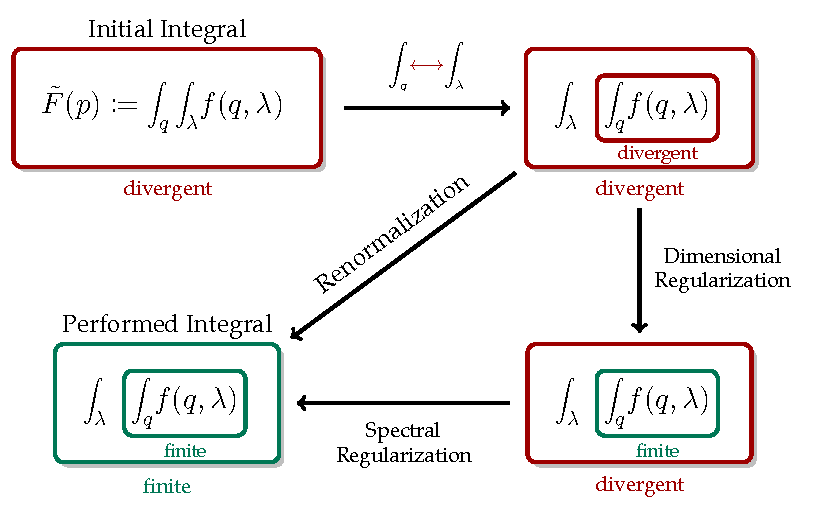
\includegraphics[width=0.8\textwidth]{figs/tikz/spectral_renormalization}
\caption[Applied regularization procedure.]{Applied regularization procedure. $f$ is some arbitrary divergent integrand. The two upper boxes have to be understood as finite by dimensional regularization but divergent in the limit $\varepsilon\rightarrow 0$. The first step consists of evaluating the momentum integral analytically using dimensional regularization \cite{Leibbrandt1975} before renormalizing the spectral integrands subsequently according to a BPHZ-renormalization scheme \cite{BogolyubovParasiuk1954, Hepp1966, Zimmermann1969}.}\label{fig:spectral_renormalization}
\end{figure}
\noindent
We will motivate the application of this scheme at the concrete example of our calculation of the quark self energy diagram, given by
\begin{align}
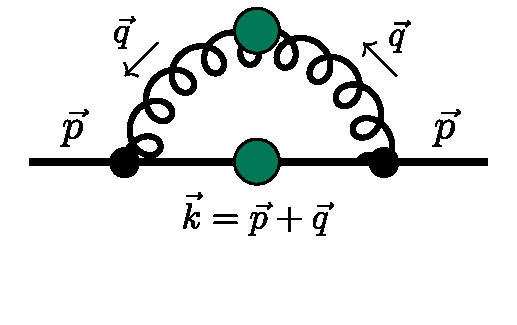
\includegraphics[scale=0.45, valign=c, trim = 0 6em 0 0]{figs/diagrams/quark_self_energy_classical} := \Sigma_q
(p) &= (-ig)^2 \delta^{ab}C_f \int_q\ \Pi^{\mu\nu}_{\perp}(q) G_A(q)\gamma_{\mu}G_q(p+q)\gamma_{\nu},
\end{align}
employing the Feynman rules for QCD in the Landau gauge. Note, that throughout this work, we will approximate the full quark-gluon vertex by its classical, bare counterpart:
 \begin{equation}
 	\Gamma^{(3)}_{q\bar{q}A} \equiv S^{(3)}_{q\bar{q}A},
 \end{equation}
leaving us with one spectral integral for the gluon and one for the quark propagator, respectively. The gluon and quark propagators are parametrized as 
\begin{align}
\left[G_{A}\right]_{\mu \nu}^{a b}&=\delta^{a b}\ \Pi_{\mu \nu}^{\perp}(p)\ G_{A}(p) + \frac{1}{\xi} \delta^{a b}\ \Pi_{\mu \nu}^{\|}(p)\ p^{2},\\
\left[G_{q}\right]^{a b} &= \delta^{ab}G_q(p),
\end{align}
with the longitudinal and transversal projectors defined as 
\begin{align}
\Pi_{\|}^{\mu \nu}(p)&=\frac{p^{\mu} p^{\nu}}{p^{2}},\\
\Pi_{\perp}^{\mu \nu}(p)&= \delta^{\mu\nu} - \Pi_{\|}^{\mu\nu}(p). \label{eqn:transversal_projector}
\end{align}
The advantage of working in Landau gauge, hence employing $\xi\rightarrow 0$, is, that it  allows for a closure of the transversal sector and the longitudinal components of the presented parameterization of the gluon propagator do not explicitly enter our calculation, cf. \cite{CyrolFisterMitterPawlowskiStrodthoff2016}. The quark DSE is projected onto $G_q$ via the application of a color trace, i.\,e. 
\begin{equation}
\left[\Gamma_{q}^{(2)}\right]^{a b}\quad \longrightarrow\quad \delta_{a b} \left[\Gamma_{q}^{(2)}\right]^{a b}.
\end{equation}
For the parts of the propagators, that are independent of the Lorentz and color structure, we insert the spectral representations
\begin{align}
G_{A}(q)&= \int_{\lambda_1}\ \frac{\lambda_1\rho_A(\lambda_1)}{q^{2}+\lambda_1^{2}},\label{eqn:GluonSpec}\\[1em]
G_q(p+q) &= -i(\slashed{p}+\slashed{q})\cdot G_{q}^{D}(p+q)+G_{q}^M(p+q)\nonumber \\
&= (\slashed{p}+\slashed{q}) \int_{\lambda_2}\ \frac{\lambda_2\rho_{q}^D(\lambda_2)}{(p+q)^{2}+\lambda_2^2}+ \int_{\lambda_2}\ \frac{\lambda_2\rho_{q}^M(\lambda_2)}{(p+q)^{2}+\lambda_2^2},\label{eqn:QuarkSpecFunc}
\end{align}
with the conventions for the spectral integrations given by
\begin{equation}
	\int_{\lambda_i} = \int_0^{\infty} \frac{\dd\lambda_i}{\pi} \qquad \text{and} \qquad \int\limits_{\left\{\lambda_i,\lambda_j\right\}} = \int_0^{\infty} \frac{\dd\lambda_i}{\pi}\frac{\dd\lambda_j}{\pi}.	 
\end{equation}
The detailed discussion on the Dirac structure of the quark propagator is moved to \appref{chap:appendixB}. For the sake of completeness, the full expression for the quark propagator in terms of the two dressing functions $Z_q(p)$ and $M_q(p)$ is given in the following:
\begin{equation}
	G_q(p) =  -i\slashed{p} \left(\frac{Z_q(p)}{p^2 + M_q^2(p)}\right) +  \left(\frac{Z_q(p)M_q(p)}{p^2 + M_q^2(p)}\right)
\end{equation}
The splitting of the quark propagator into two distinct parts, referred to as Dirac vector ($\sim i\slashed{p}$) and Dirac scalar ($\sim\mathbb{1}$) part, respectively, allows for a separation of the calculation of the diagram according to
\begin{equation}
	\Sigma_q(p) =\slashed{p}\cdot\Sigma_{q}^D(p) + \Sigma_{q}^M(p),
\end{equation}
leading us to two independent integral equations, i.\,e.
\begin{align}
\Sigma_{q}^D(p) &= (-ig)^2\delta^{ab}C_f\int\limits_{\left\{\lambda_1,\lambda_2\right\}}\lambda_1\lambda_2\rho_A(\lambda_1)\rho_q^D(\lambda_2)\cdot I_q^D\left(p, \lambda_1, \lambda_2,x\right),\\
\Sigma_{q}^M(p) &= (-ig)^2\delta^{ab}C_f\int\limits_{\left\{\lambda_1,\lambda_2\right\}}\lambda_1\lambda_2\rho_A(\lambda_1)\rho_q^M(\lambda_2)\cdot I_q^M\left(p, \lambda_1, \lambda_2,x\right).
\end{align}
As already mentioned before, we will \textit{not} display the full, lengthy analytic expressions for the integrands here, but in \appref{chap:appendixA}. \\
Note, that we already implicitly performed the first non-trivial step of the calculation, which consists of swapping the integration order $q\leftrightarrow\{\lambda_1,\lambda_2\}$, corresponding to the step from upper left to the upper right box in \figref{fig:spectral_renormalization}. This is only valid for the case, that both integrations are finite by themselves according to Fubinis theorem. At this point, the finiteness of both integrations is explicitly assumed.\\
By naive power counting, we directly see that the considered diagram is superficially divergent. This requires us to set up a suitable regularization procedure for the integrands in order to proceed with the calculation. For the first part of the calculation, the loop momentum integration is rendered finite by means of dimensional regularization, hence the integrands are evaluated for $d= 4 -2\varepsilon$ and expanded up to lowest order in the limit $\varepsilon\rightarrow 0$. This isolates the divergence of the diagram in the 1/$\varepsilon$-term, which is discarded, as usual. The applicability of dimensional regularization comes with many advantages since it respects all space-time, internal and gauge symmetries of the theory at hand, in contrast to other regularization schemes, that require for example the introduction of explicit cutoffs.  \\
However, the remaining spectral integrands are a priori still \textit{not} finite simply by discarding the 1/$\varepsilon$-term,  which is a remnant of initially swapping the integration order. We are left with finite spectral integrands for $\varepsilon >0$, that in general need to be computed numerically. For numerical performance it is helpful to perform the spectral integrations at $\varepsilon=0$. The same is true for the access to the analytical momentum structure needed to extract the Minkowski properties. It is therefore required to set up a suitable renormalization procedure for the integrands in the limit $\varepsilon\rightarrow 0$. 
 This problem can be resolved by extending the standard dimensional regularization procedure by introducing additional counterterms on the level of the classical action, that cancel the leading and subleading divergent contributions to the spectral integrands.\\ Technically this is implemented by subtracting a Taylor expansion in all momenta around the renormalization group scale $\mu$\footnote{The integrand already depends inherently on the RG scale $\mu$ due to dimensional regularization. \\}, which modifies the UV behavior of the integrand to drop off faster\footnote{We have to cope with the fact, that  the underlying BPHZ-scheme in general does not preserve all symmetries of a given theory and in particular breaks gauge symmetry, but this is also true for other subtraction schemes that introduce explicit counterterms, while leading to  gauge-consistent results.}.  This procedure is called spectral BPHZ-renormalization, cf. \cite{HorakPawlowskiWink2020, BogolyubovParasiuk1954,Hepp1966,Zimmermann1969}. 
 For a schematic overview, cf. \figref{fig:BPHZ}. We visualized the explicit effects of this procedure on the respective integrands in the appendix in \figref{fig:BPHZ_demonstration}.
 The introduced counterterms therefore explicitly contribute to the mass renormalization $M_q(p)$ as well as to the wave function renormalization $Z_q(p)$, characterizing the momentum dependence of the quark propagator, cf. \appref{chap:appendixB} for a detailed discussion. The counterterms consistently remove the divergent parts of the integrands and we explicitly checked for UV-finiteness of all integrations. This finally allows us to solve the spectral integrals numerically after successfully performing the limit $\varepsilon\rightarrow 0$ beforehand.
 \begin{figure}[t]
	\centering
	\begin{align*}
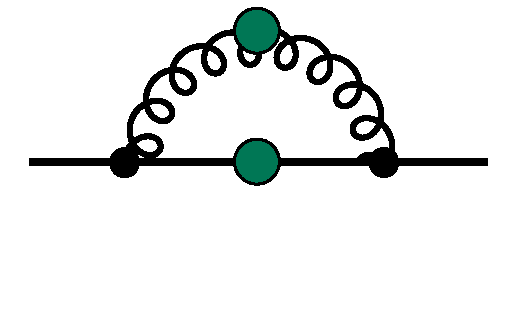
\includegraphics[scale=0.28, valign=c]{figs/diagrams/bphz/quark_self_energy_classical} \longrightarrow 
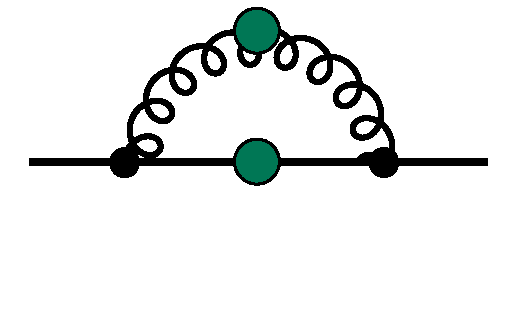
\includegraphics[scale=0.28, valign=c]{figs/diagrams/bphz/quark_self_energy_classical} - \eval{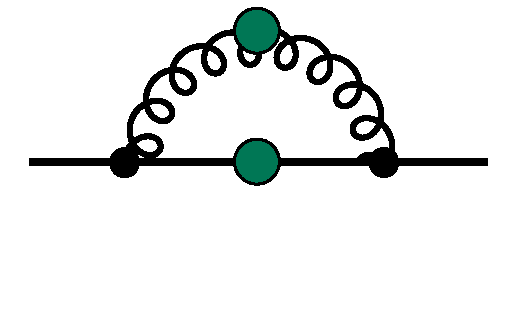
\includegraphics[scale=0.28, valign=c]{figs/diagrams/bphz/quark_self_energy_classical}}_{p=\mu} -\ \frac{(p^2-\mu^2)}{2\mu}\left[\partial_{p}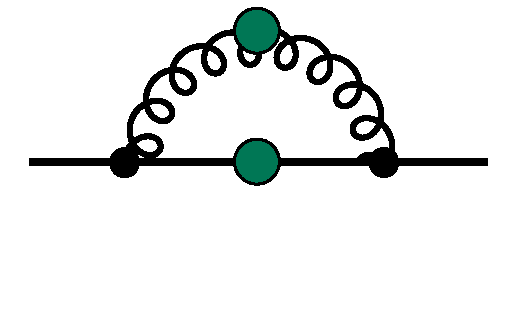
\includegraphics[scale=0.28, valign=c]{figs/diagrams/bphz/quark_self_energy_classical}\right]_{p=\mu}
\end{align*}

	\caption[Schematic spectral BPHZ-renormalization procedure at the example of the quark self energy diagram.]{Schematic spectral BPHZ-renormalization procedure at the example of the quark self energy diagram. The diagram is subtracted by the first two terms of its own Taylor expansion around the RG scale $\mu$ in order to cancel quadratic and logarithmic divergences of the spectral integrands. For a demonstration of the actual effects of the subtraction scheme on the spectral integrands, we refer to \figref{fig:BPHZ_demonstration} in the appendix.} 
	\label{fig:BPHZ}
\end{figure}
Note, that although this might seem like two separate regularization procedures, the above subtraction scheme really just corresponds to the correct application of dimensional regularization. Technically this corresponds to evaluating the integrals at some point $\alpha$ in the complex exponent plane, where the integration is finite. Afterwards all terms are expanded in a Laurent series around $\alpha=d$, and subtracting the first term of this series removes all singularities of this construction by employing finite renormalization conditions. This naturally discards the divergent parts of the spectral integrals, as they depend on the dimension $d$ \cite{Leibbrandt1975, Horak2019}.
In a last step, the (now appropriately regularized) Euclidean expressions can be analytically continued to the real momentum axis according to 
\begin{equation}
	I_q^{(D/M)}\left(\omega, \lambda_1, \lambda_2\right) := I_q^{(D/M)}\left(-i(\omega + i0^+)\right).
\end{equation}
This needs to be done, since the spectral functions are obtained from the retarded propagator. For a visualization, cf. \figref{fig:continuation}.

\section{Iterative Procedure}
With the finite Euclidean and real-time expressions for the spectral integrands $I_q^{(D/M)}(p/\omega)$ at hand, the DSE is now solved iteratively, by performing the spectral integrations and extracting the spectral functions $\rho_q^{(D/M)}$ from the respective parts of the retarded propagator via \eqref{eqn:specfunc_relation}, or to be more precise via \eqref{eqn:correct_relation}. The updated result for the quark spectral functions are then fed back into the computation of the diagram until convergence of the result (by eyesight) is observed. A detailed overview of our numerical workflow is depicted in \figref{fig:numerics}. For explicit details concerning the numerical implementation, we refer to \appref{chap:appendixC}.\\
\begin{figure}[t]
	%\centering
	\hspace{-4.5em}
	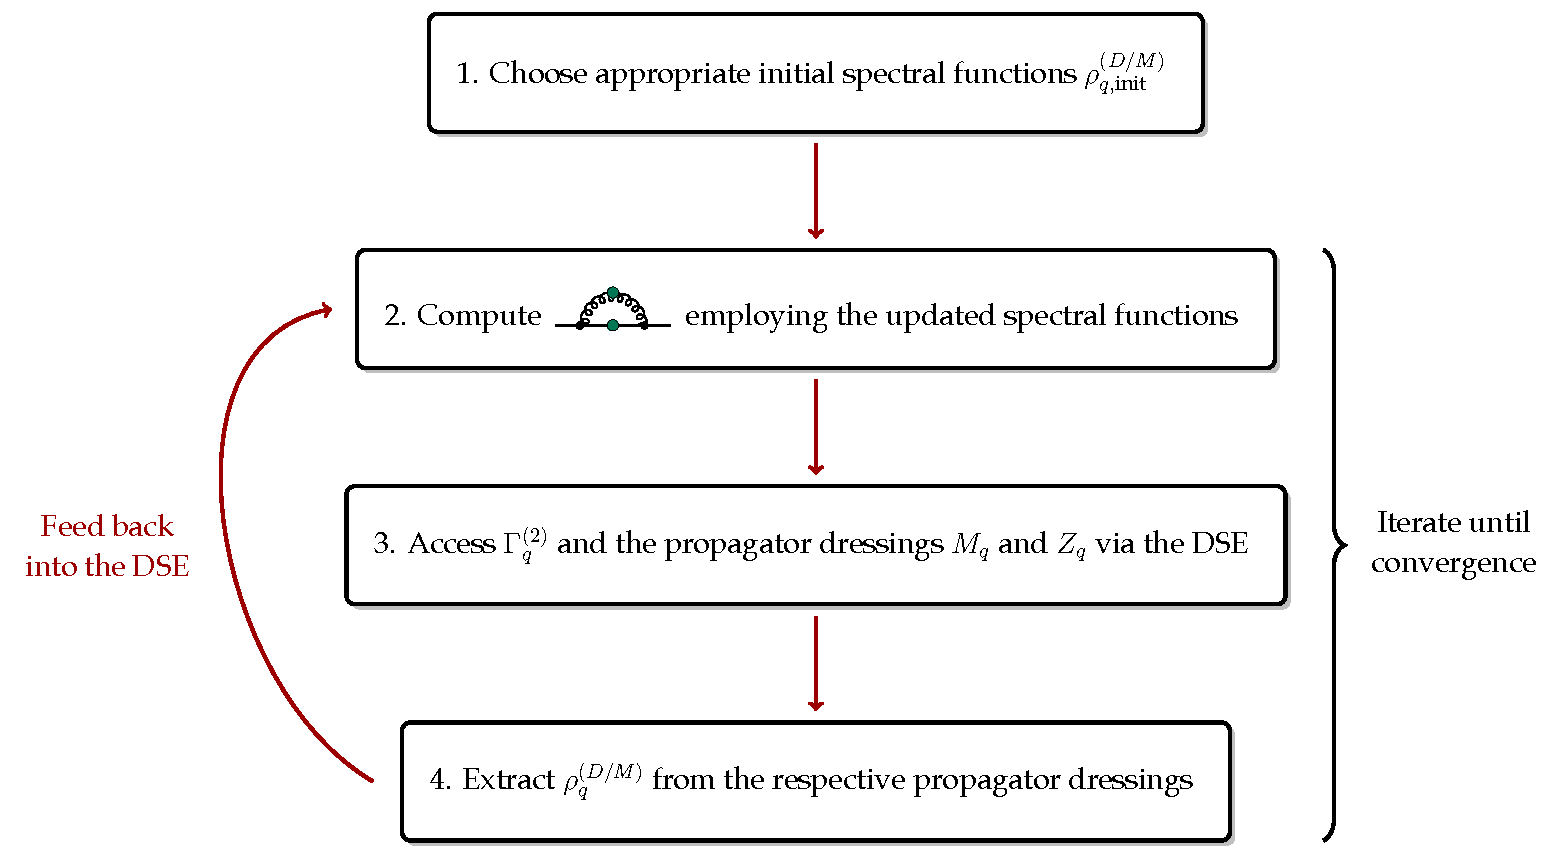
\includegraphics[width = 1.2\textwidth]{figs/tikz/iterative_computation}
	\caption{Iterative procedure to extract the spectral function from the DSE.} 
	\label{fig:numerics}
\end{figure}
Before starting the iterative procedure, appropriate initial \enquote{guesses} for both quark spectral functions $\rho_q^D(\lambda_2)$ and $\rho_q^M(\lambda_2)$ have to be made. A well motivated guess for the quark spectral functions is to employ quasi-classical spectral functions, reproducing  the classical, perturbative quark propagator. They are simply given by (massive) delta distributions:
	\begin{align}
		\rho_{q,\mathrm{init}}^D(\lambda) &= 2\pi i\ \frac{\delta(\lambda-m_q)}{2\lambda}\\
		\rho_{q,\mathrm{init}}^M(\lambda) &= 2\pi m_q\ \frac{\delta(\lambda-m_q)}{2\lambda}.
	\end{align}
The gluon input is considered as \enquote{static} in our computation. The gluon spectral function $\rho_A$ of our choice is given analytically and does not need to be updated after every iteration step. For this concrete example, $\rho_A$ was obtained in \cite{CyrolPawlowskiRothkopWink2018} by reconstruction from numerical data for the Euclidean gluon propagator. This specific result for the gluon spectral function respects the so called \textit{decoupling} (or \textit{massive}) solution for the gluon propagator in the infrared \cite{vonSmekalAlkoferHauck1997}. In future studies, this might be adapted to solutions respecting the known \textit{scaling scenario} \cite{LercheVonSmekal2002}, which has been found to provide a dynamical generation of a mass gap for both the gluon and the ghost propagators, but is in general more complicated due to the non-trivial scaling exponent $\kappa$ with $\frac{1}{2}<\kappa < 1$, slighty modifying the explicit IR behavior .
For a visualization of the chosen gluon spectral function and the corresponding gluon propagator, cf. \figref{fig:gluon_specfunc_and_prop}.
\begin{figure}[t]
\hfill
	\centering
	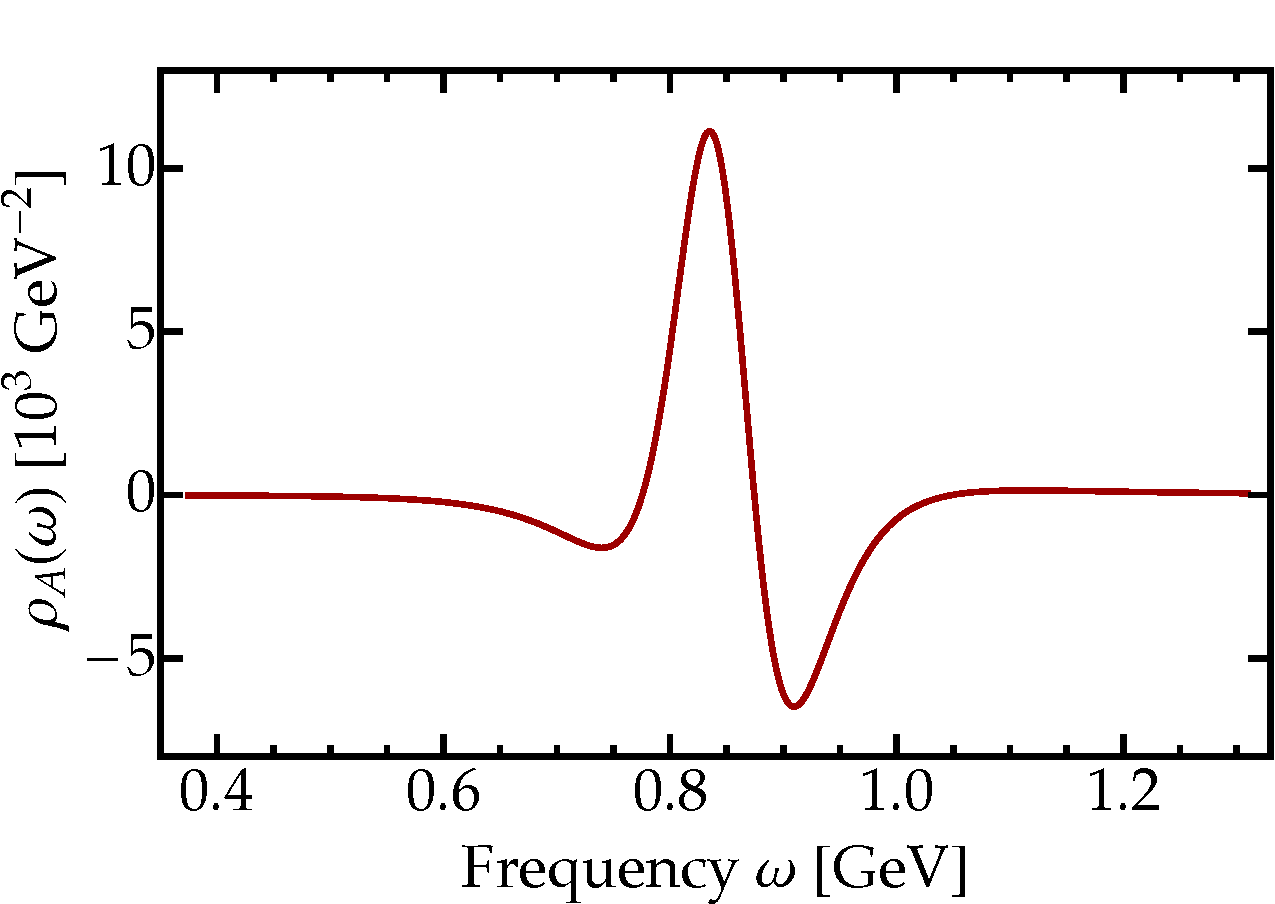
\includegraphics[width = 0.46\textwidth, trim= 4em 0 0 0]{figs/plots/GluonSpecFuncPlot}
\hfill
	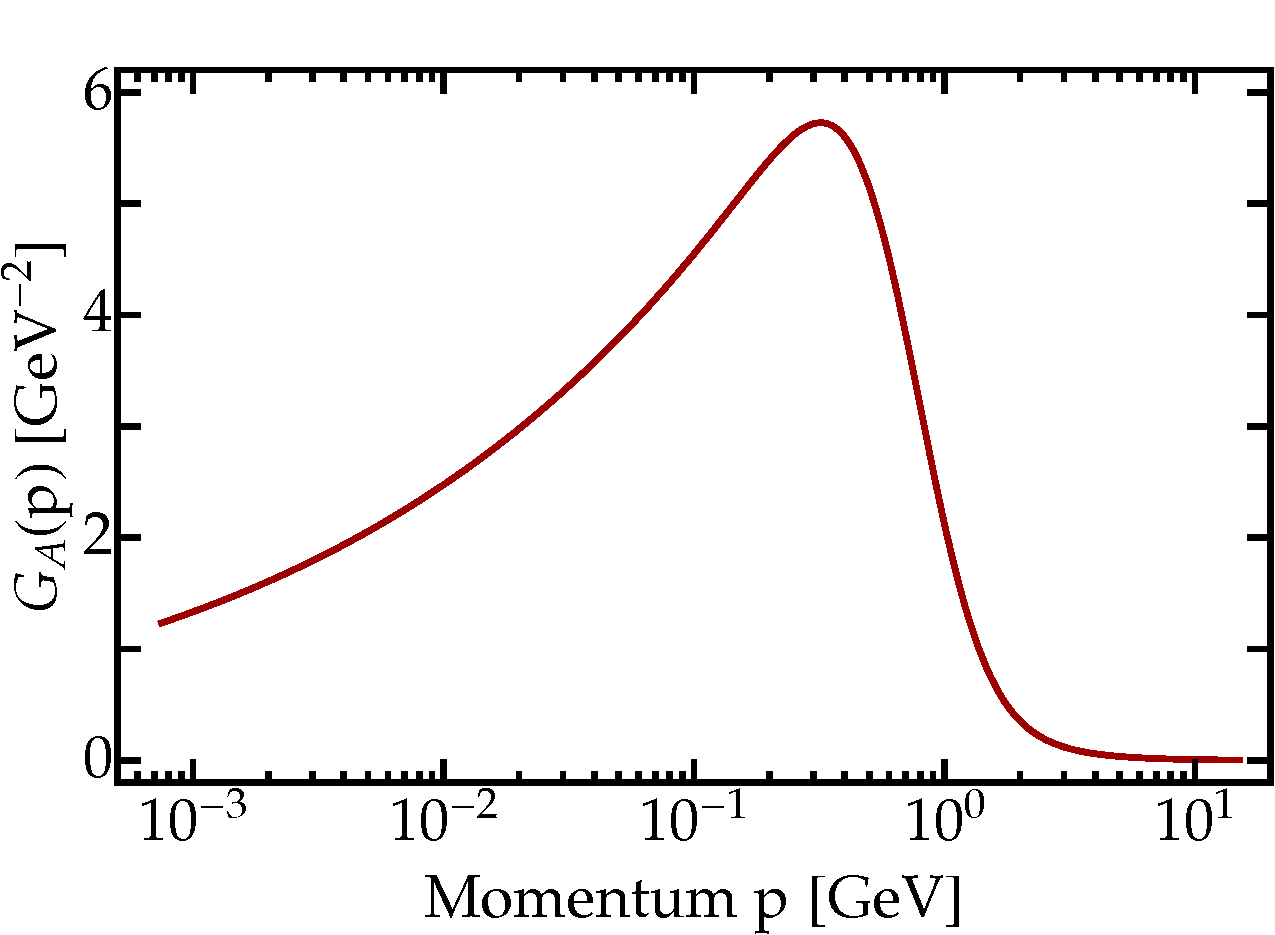
\includegraphics[width = 0.445\textwidth, trim= 4em 0 0 0]{figs/plots/GluonPropPlot}
\hfill
	\caption[Chosen input gluon spectral function and corresponding propagator.]{Chosen input gluon spectral function (left) and the corresponding propagator obtained from \eqref{eqn:GluonSpec} (right). This spectral function was determined in \cite{CyrolPawlowskiRothkopWink2018} by reconstructing numerical FRG data.}
\label{fig:gluon_specfunc_and_prop}
\end{figure}
This completes our presentation of the conducted calculations, the results for the spectral functions and all associated quantities are presented in the following section.

\section{Results and Implications}
This last section of the main part is devoted to the discussion of our results. The relevant quantities that are computed for every iteration step according to the iterative procedure presented in \figref{fig:numerics}, are the final expressions for the Dirac vector and scalar parts of the quark self energy diagram and the dressing functions $Z_q(p)$ and $M_q(p)$, that are accessed via the quark propagator DSE. Each of these quantities has been evaluated for Euclidean as well as real-time momenta/frequencies. The results shown in the following are obtained by interpolating the discrete expressions, that were obtained by computing the numerical integrals on a discrete momentum grid. Again, we refer to \appref{chap:appendixC} for further details concerning the numerical implementation. \\The results for the computed  dressing functions for different iteration steps are displayed in \figref{fig:computed_dressings}, at the beginning of the next page. Note, that the initially arbitrary momentum scales can be converted into actual physical units via the peak position of the input gluon spectral function, which has been determined in lattice studies to be at around 1 GeV. 
 Qualitatively, the results for the iterated dressing functions look very stable, already for a small number of iterations. The wave function renormalization tends to one in the IR and to zero in the UV with a rather smooth transition in the range from 10 to $10^2$ GeV. This specific form hints at a problem with the finiteness of the Dirac vector part in our computation. From its definition as $Z_q(p)=1/A(p)$, where $A(p)$ collects all parts of the quark DSE, that are $\sim i\slashed{p}$, it looks like the value of the Dirac vector part of the diagram tends to infinity, hence explaining the value of zero in $Z_q(p)$.  This problem could not be resolved yet upon completion of this thesis.\\
The quark mass function $M_q(p)$ also exhibits a stable IR and UV behavior, tending to a finite value of $\sim 0.38$ GeV in the IR. We observe a characteristic negative dip in the region of 1 GeV up to $10^2$ GeV, that should not be present, since the mass function should be a positive quantity. This could be related to the problem concerning $Z_q(p)$, which is also visible in the UV limit of the mass function where it tends to zero. This is expected from the properties of $Z_q(p)$, since it enters the computation of $M_q(p)=B(p)/A(p)=Z(p)B(p)$ as a multiplicative factor and therefore cancels out all non-zero contributions to $M_q(p)$ in the UV.
 \begin{figure}[t] 
\hfill
	\centering
	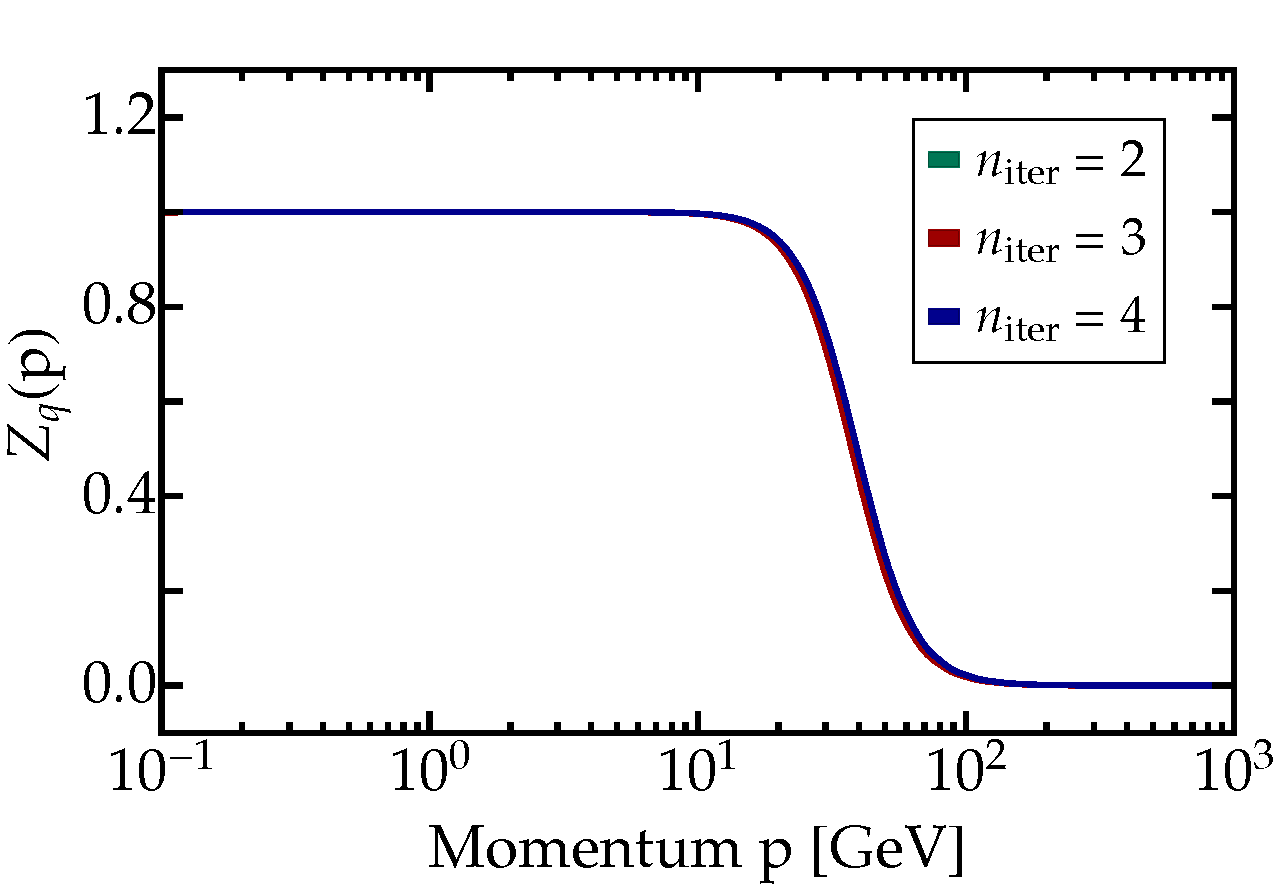
\includegraphics[width = 0.46\textwidth, trim= 4em 0 0 0]{figs/plots/ZqPlot}
\hfill
	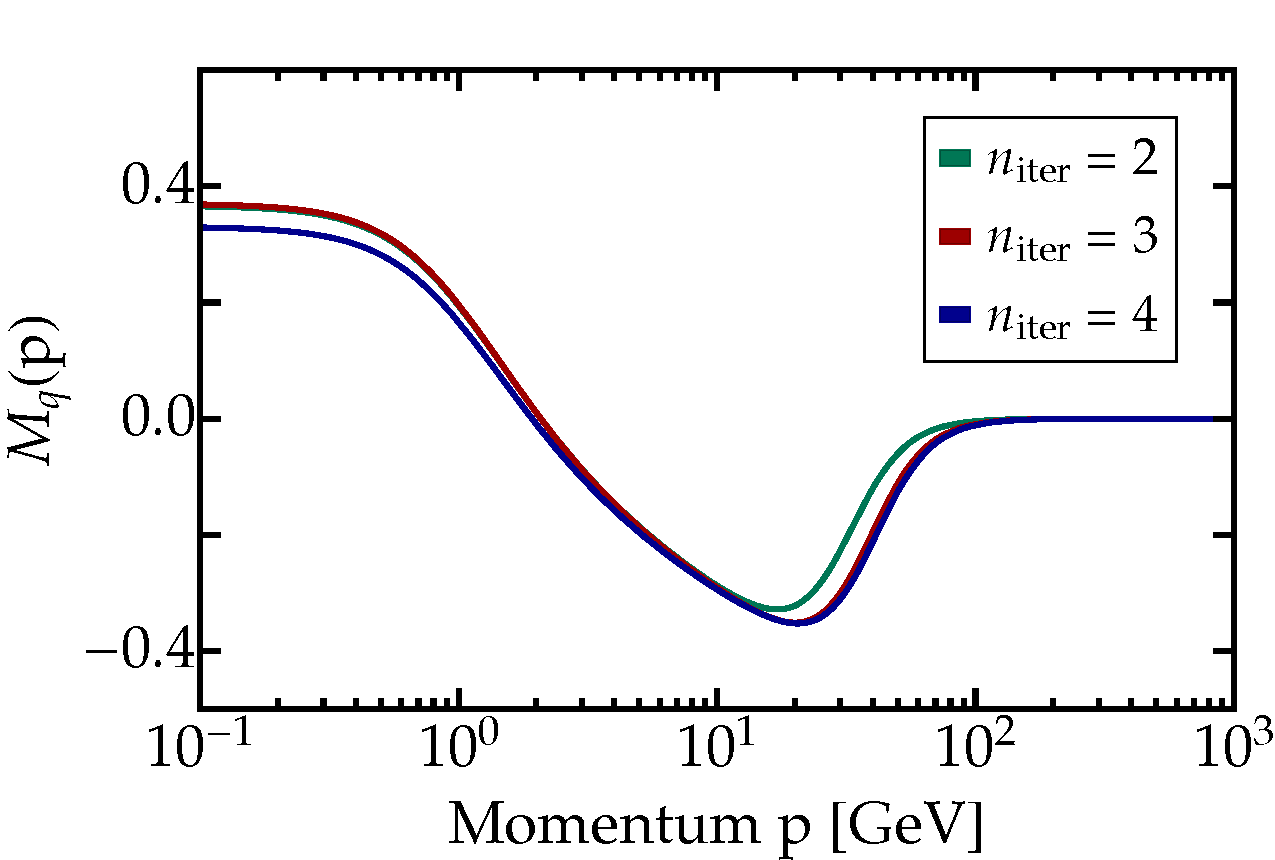
\includegraphics[width = 0.475\textwidth, trim= 4em 0 0 0]{figs/plots/MqPlot}
\hfill
	\caption[Computed quark propagator dressings $Z_q(p)$ and $M_q(p)$.]{Computed quark propagator dressings $Z_q(p)$ and $M_q(p)$ for different iteration steps.}
\label{fig:computed_dressings}
\end{figure}

The results for the quark spectral functions $\rho_q^D(\omega)$ and $\rho_q^M(\omega)$ are displayed in \figref{fig:specfunc_results} at the beginning of the next page. The development of the typical peak structure is clearly visible. The spectral functions feature negative regions, which might at first seem to be in contradiction with the probabilistic interpretation discussed in \chapref{chap:methods}. Upon further consideration however, this is also observed in other scenarios, such as for example for the gluon input we are using in this work. A possible explanation could be, that the two spectral functions associated with the quark propagator are no spectral functions of an actual observable particle and therefore are not necessarily required to obey positivy.  Nevertheless, no convergent solution for the iterative procedure could be found. As a benchmark check, we show the corresponding parts of the Euclidean propagator computed directly from the DSE, highlighted in blue, and from the spectral functions via \eqref{eqn:correct_relation}, highlighted in red. No exact agreement is observed and hence, the spectral representation is violated. This is another hint at a possible problem with the used input for the iterative procedure. Note, that as soon as the spectral representation is violated, the iterative solution procedure immediately breaks down, as \eqref{eqn:correct_relation} no longer holds. Starting from the above set of input parameters, the iteration runs into an unstable direction where the spectral representation does not hold for the quark propagators. To conclude this discussion we remark, that if there exists a solution to the quark DSE respecting the spectral representation, the initial conditions have to be closer to the actual solution, i.\,e. in the basin of attraction. Additionally, the observed discrepancies hint at an error in the calculation of the relevant diagram, that was not found  upon completion of this thesis. 
 
 \begin{figure}[t] 
\hfill
	\centering
	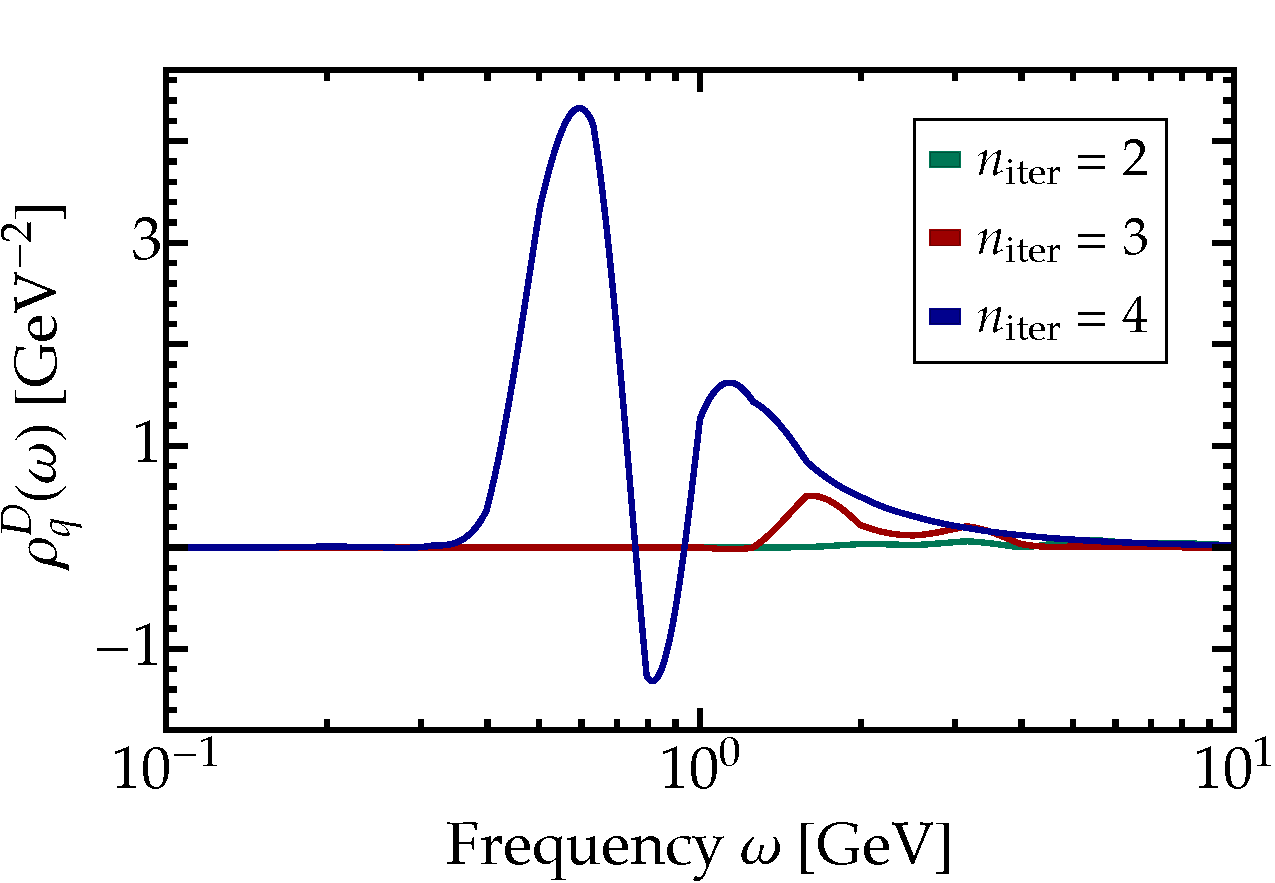
\includegraphics[width = 0.48\textwidth, trim= 4em 0 0 0]{figs/plots/rhoqDPlot}
\hfill
	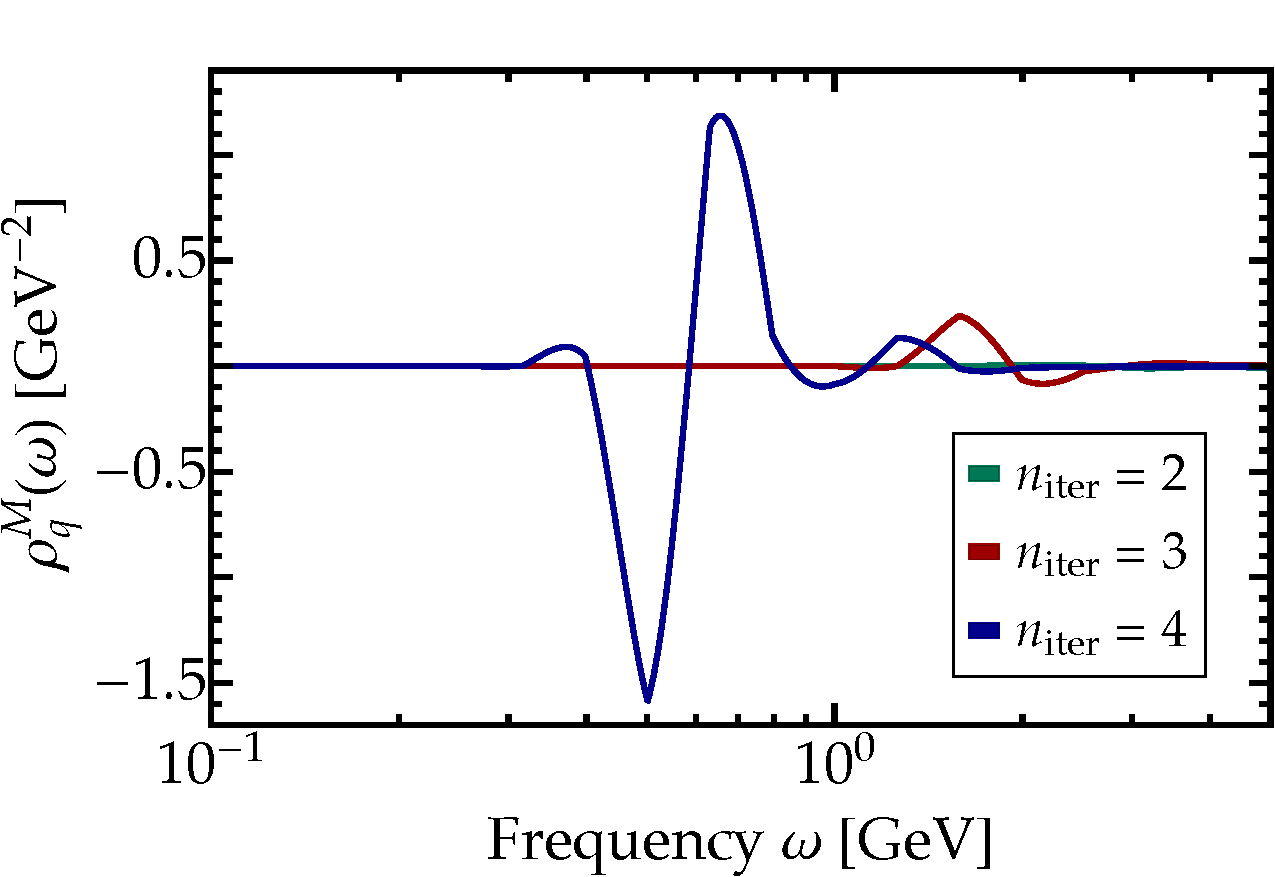
\includegraphics[width = 0.48\textwidth, trim= 4em 0 0 0 0]{figs/plots/rhoqMPlot}
\hfill \\
\hfill
	\centering
	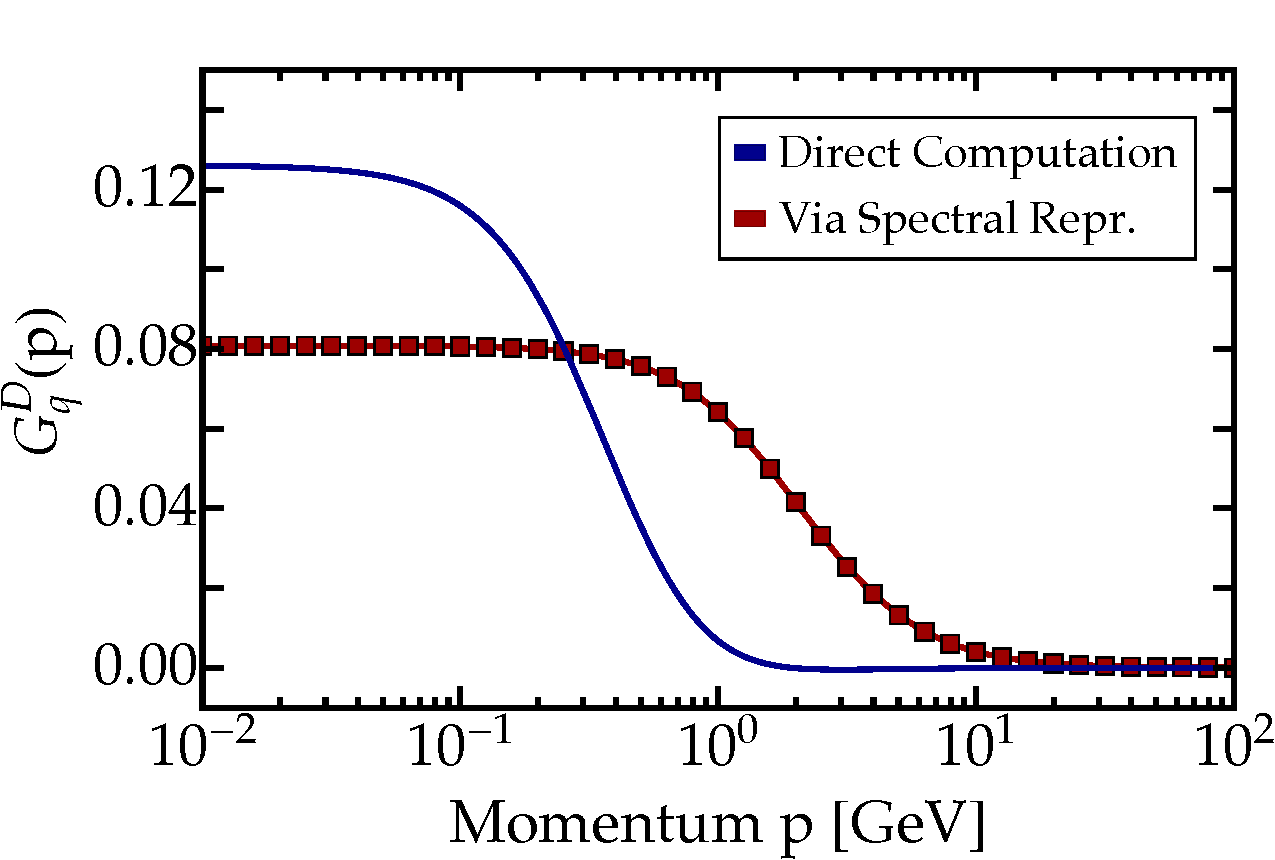
\includegraphics[width = 0.485\textwidth, trim= 3em 0 0 0]{figs/plots/BenchmarkPlotVec}
\hspace{0.5em}
	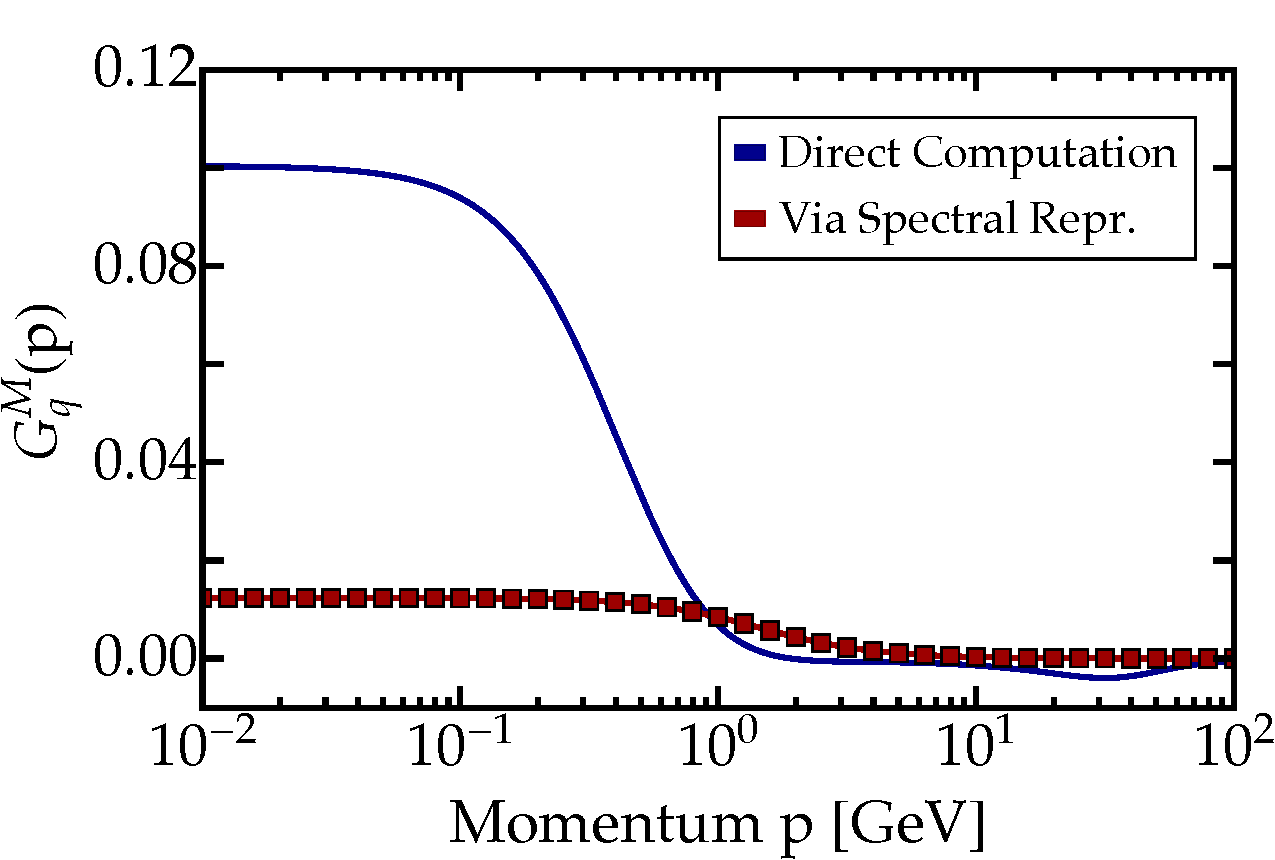
\includegraphics[width = 0.485\textwidth, trim= 3em 0 0 0]{figs/plots/BenchmarkPlotScal}
\hfill
	\caption[Computed quark spectral functions $\rho_q^D(\omega)$ and $\rho_q(\omega)$ and corresponding propagator dressings.]{First row: Computed quark spectral functions $\rho_q^D(\omega)$ and $\rho_q^M(\omega)$ for different numbers of iterations. Second row: Comparison of the respective parts of the Euclidean quark propagator with the result obtained by the spectral representation given in \eqref{eqn:QuarkSpecFunc} for the last iteration step $n_{\mathrm{iter}}=4$.}
\label{fig:specfunc_results}
\end{figure}

